\documentclass[tikz, border=10pt]{standalone}

% % -*- root: ../main.tex -*-

\definecolor{jgu_rot}{RGB}{193,0,42}
\definecolor{jgu_hellgrau}{RGB}{172,172,172}
\definecolor{jgu_dunkelgrau}{RGB}{99,99,99}
\definecolor{matlab_blau}{rgb}{0.00000,0.44700,0.74100}
\definecolor{matlab_orange}{rgb}{0.85000,0.32500,0.09800}

% matlab colors
\definecolor{mycolor1}{rgb}{0.00000,0.44700,0.74100}%
\definecolor{mycolor2}{rgb}{0.85000,0.32500,0.09800}%
\definecolor{mycolor3}{rgb}{0.92900,0.69400,0.12500}%
\definecolor{mycolor4}{rgb}{0.49400,0.18400,0.55600}%
\definecolor{mycolor5}{rgb}{0.46600,0.67400,0.18800}%


\begin{document}
    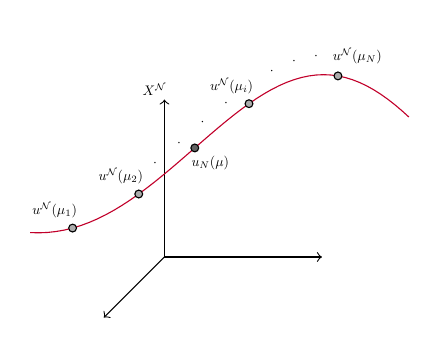
\begin{tikzpicture}[
      declare function={
        fx(\x) = \x;
        fy(\x) = 1 + sin(\x*50);
        fz(\x) = -cos(\x*20);
      },
      every node/.style={
        draw,
        shape=circle,
        scale=0.5,
        inner sep=2pt,
        outer sep=-2pt
      },
      % x={(1cm,0cm)},
      % y={(0cm,1cm)},
      % z={(-1cm,-1cm)}
    ]

      % Achsen
      \draw [->] (0,0,0) -- (2,0,0); % node[right] {};
      \draw [->] (0,0,0) -- (0,2,0) node[above left, draw=none] {$X^{\mathcal N}$};
      \draw [->] (0,0,0) -- (0,0,2); % node[above] {};

      % Kurve
      \draw [jgu_rot] ({fx(-2)}, {fy(-2)}, {fz(-2)})
      \foreach \x in {-2,-1.9,...,3}
      { -- ({fx(\x)}, {fy(\x)}, {fz(\x)})
      };

      % RB-Punkte
      \draw ({fx(-1.5)}, {fy(-1.5)}, {fz(-1.5)}) node [label=above left:$u^{\mathcal N}(\mu_{1})$,fill=jgu_hellgrau] {};
      \draw ({fx(-0.7)}, {fy(-0.7)}, {fz(-0.7)}) node [label=above left:$u^{\mathcal N}(\mu_{2})$,fill=jgu_hellgrau] {};
      \draw ({fx(0.7)}, {fy(0.7)}, {fz(0.7)}) node [label=above left:$u^{\mathcal N}(\mu_{i})$,fill=jgu_hellgrau] {};
      \draw ({fx(1.9)}, {fy(1.9)}, {fz(1.9)}) node [label=above right:$u^{\mathcal N}(\mu_{N})$,fill=jgu_hellgrau] {};

      % FE-Punkt
      \draw ({fx(0)}, {fy(0)}, {fz(0)}) node [label=below right:$u_{N}(\mu)$,fill=jgu_dunkelgrau] {};

      % Dots
      \draw ({fx(-0.5)}, {fy(-0.5)}, {fz(-0.5)}) node [draw=none,fill=none,label=above:$\cdot$,outer sep=7pt] {};
      \draw ({fx(-0.2)}, {fy(-0.2)}, {fz(-0.2)}) node [draw=none,fill=none,label=above:$\cdot$,outer sep=7pt] {};
      \draw ({fx(0.1)}, {fy(0.1)}, {fz(0.1)}) node [draw=none,fill=none,label=above:$\cdot$,outer sep=7pt] {};
      \draw ({fx(0.4)}, {fy(0.4)}, {fz(0.4)}) node [draw=none,fill=none,label=above:$\cdot$,outer sep=7pt] {};
      \draw ({fx(1.0)}, {fy(1.0)}, {fz(1.0)}) node [draw=none,fill=none,label=above:$\cdot$,outer sep=7pt] {};
      \draw ({fx(1.3)}, {fy(1.3)}, {fz(1.3)}) node [draw=none,fill=none,label=above:$\cdot$,outer sep=7pt] {};
      \draw ({fx(1.6)}, {fy(1.6)}, {fz(1.6)}) node [draw=none,fill=none,label=above:$\cdot$,outer sep=7pt] {};
    \end{tikzpicture}
\end{document}
